\documentclass[11pt]{amsart}
\usepackage[marginratio=1:1, margin=0.8in]{geometry}  % See geometry.pdf to learn the layout options. There are lots.
%\geometry{a4paper} % ... or a4paper or a5paper or ... 
%\geometry{landscape}                % Activate for for rotated page geometry
%\usepackage[parfill]{parskip}    % Activate to begin paragraphs with an empty line rather than an indent
%\usepackage{graphicx}
% \usepackage{amssymb}
\usepackage{palatino}
\usepackage{natbib}
\usepackage[parfill]{parskip} 
\usepackage{caption}
\usepackage{subcaption}

\usepackage{tikz}
\usepackage{pgf}
\usepackage{tkz-graph}

\newtheorem{theorem}{Theorem}
\newtheorem{lemma}[theorem]{Lemma}

\theoremstyle{definition}
\newtheorem{definition}{Definition}

\theoremstyle{question}
\newtheorem{question}{Question}


\title[HBS 4403: Management Control and Performance Measurement]{HBS 4403: Problem Set 2}

\author{Ian D. Gow}
%\email{igow@hbs.edu}

\begin{document}
\usetikzlibrary{automata, shapes, calc, positioning}
\maketitle
% \date{}

\bibliographystyle{chicago}

The goal of this problem set is to help you gain some proficiency in applying the back-door criterion discussed in Chapter 4 of \citet{Morgan:2014vg}. 
The following definitions come from \citet{Pearl:2009vo}, which is a bit more mathematical than \citet{Morgan:2014vg}.

% Some definitions and a theorem ----
\begin{definition}[$d$-separation, block, collider]
A path $p$ is said to be \emph{$d$-separated} (or \emph{blocked}) by a set of nodes $Z$ if and only if
\begin{enumerate}
	\item $p$ contains a chain $i \rightarrow m \rightarrow j$ or a fork $i \leftarrow m \rightarrow j$ such that the middle node $m$ is in $Z$, or
	\item $p$ contains an inverted fork (or \emph{collider}) $i \rightarrow m \leftarrow j$ such that the middle node $m$ is not in $Z$ and such that no descendant of $m$ is in $Z$
\end{enumerate}
\end{definition}

\begin{definition}[Back-door criterion]
A set of variables $Z$ satisfies the \emph{back-door criterion} relative to a an ordered pair of variables $(X, Y)$ in a 
	DAG $G$ if:
	\begin{itemize}
		\item no node in $Z$ is a descendant of $X$; and
		\item $Z$ blocks every path between $X$ and $Y$ that contains an arrow into $X$.\footnote{The ``arrow into $X$" is the portion of the definition that is explains the ``back-door" terminology.}
	\end{itemize}
\end{definition}

Given these definitions, \citet[p.\,79]{Pearl:2009vo}
proves the following result.
\begin{theorem}[Back-door adjustment]
	If a set of variables $Z$ satisfies the back-door criterion relative to $(X, Y)$, then the causal effect of $X$ on $Y$ is identifiable and is given by the formula 
	\[ P(y | x) = \sum_{z} P(y | x, z) P(z), \]
where $P(y|x)$ stands for the probability that $Y = y$, given that $X$ is set to level $X=x$ by external intervention.\footnote{
How the quantities $P(y|x)$ map into estimates of causal effects is not critical to the current assignment, it suffices to note that in a given setting, it can be calculated if the needed variables are observable.}
\end{theorem}

% The causal diagram ----
\begin{figure}[h]
	\caption{Causal diagram $G$} \label{fig:causal}
    \centering
    
    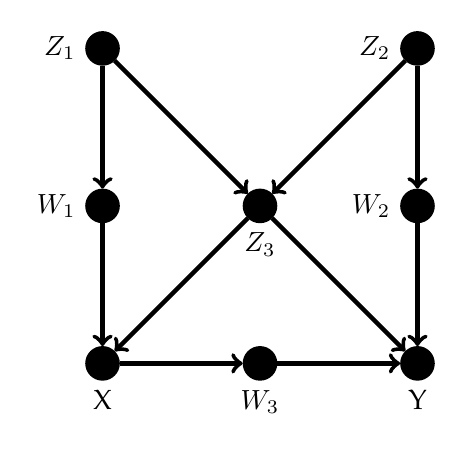
\begin{tikzpicture}
		\GraphInit[vstyle=Classic]
		\SetGraphUnit{2}
		
		% Set up the vertices (random variables)
		\Vertex[Lpos=-90]{X}
		\EA[Math,Lpos=-90](X){W_3}
		\EA[Lpos=-90](W_3){Y}
		\NO[Math,Lpos=-180](X){W_1}
		\EA[Math,Lpos=-90](W_1){Z_3}
		\NO[Math,Lpos=-180](W_1){Z_1}
		\NO[Math,Lpos=-180](Y){W_2}
		\NO[Math,Lpos=-180](W_2){Z_2}
		
		% Add the arrows
		\SetUpEdge[style={->,ultra thick},color=black]
		\Edge(X)(W_3)
		\Edge(W_2)(Y)
		\Edge(Z_3)(Y)
		\Edge(W_3)(Y)
		\Edge(W_1)(X)
		\Edge(Z_1)(W_1)
		\Edge(Z_1)(Z_3)
		\Edge(Z_2)(Z_3)
		\Edge(Z_2)(W_2)
		\Edge(Z_3)(X)
		\SetVertexNoLabel
	\end{tikzpicture}  

\end{figure}

% The questions ----
\begin{question}
Identify \emph{each} of the back-door paths into $X$ from $Y$ in graph $G$ shown in Figure \ref{fig:causal}. (\emph{Hint:} There are three, one of which is $X \leftarrow Z_3 \rightarrow Y$.)
\end{question}

\begin{question}
Which of the following sets block all back-door paths?
	\begin{itemize}
		\item $\{ W_1, Z_3 \}$
		\item $\{ W_2, Z_3 \}$
		\item $\{ Z_2, Z_3 \}$
		\item $\{ Z_3 \}$
		\item $\{ W_3 \}$
	\end{itemize}
For the sets that do not block all back-door paths, identify which paths are unblocked.
\end{question}

\bibliography{dba}

\end{document}
